We constructed a discrete coordinate system ranging from $-5R_0$ to $5R_0$ along each coordinate axis divided into $7\cross 7\cross 7$ coordinate points, and calculated the magnetic field of a dipole at the origin in these points using our implementation of eq. \ref{eq:dipoleField}. The resulting field with the corresponding dipole moment is presented in 3D in Figure \ref{fig:dipoleField}, and the planes through the origin are plotted in 2D in Figure \ref{fig:dipolePlanes}\\

\begin{figure}[ht]
    \centering
    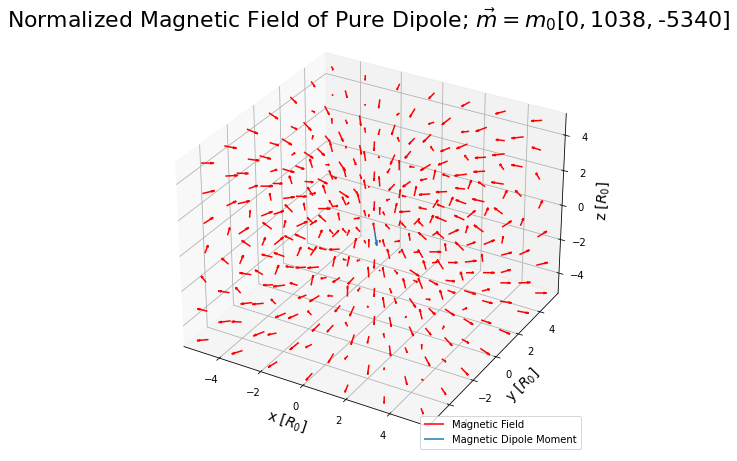
\includegraphics[scale=.4]{Images/dipoleField.png}
    \caption{Plot of the magnetic field of a pure dipole without magnitude and its corresponding magnetic dipole moment.}
    \label{fig:dipoleField}
\end{figure}

\noindent It can be observed in Figure \ref{fig:dipoleField} that the dipole field has azimuthal symmetry around an axis along the dipole moment and that the field lines point from the magnetic north to the magnetic south, which is exactly how a magnetic dipole behaves. This plot does not portray strength, only direction.\\
\\
We study the field further by assessing the $xz$-plane and $yz$-plane through the origin in shown in Figure \ref{fig:dipolePlanes}. Since the differences in magnetic field strength vary a lot with distance from the source, the strength in Figure \ref{fig:dipolePlanes} has been cut off at $1000B_0$, meaning differences near the center are not discernible.\\

\begin{figure}[ht]
    \centering
    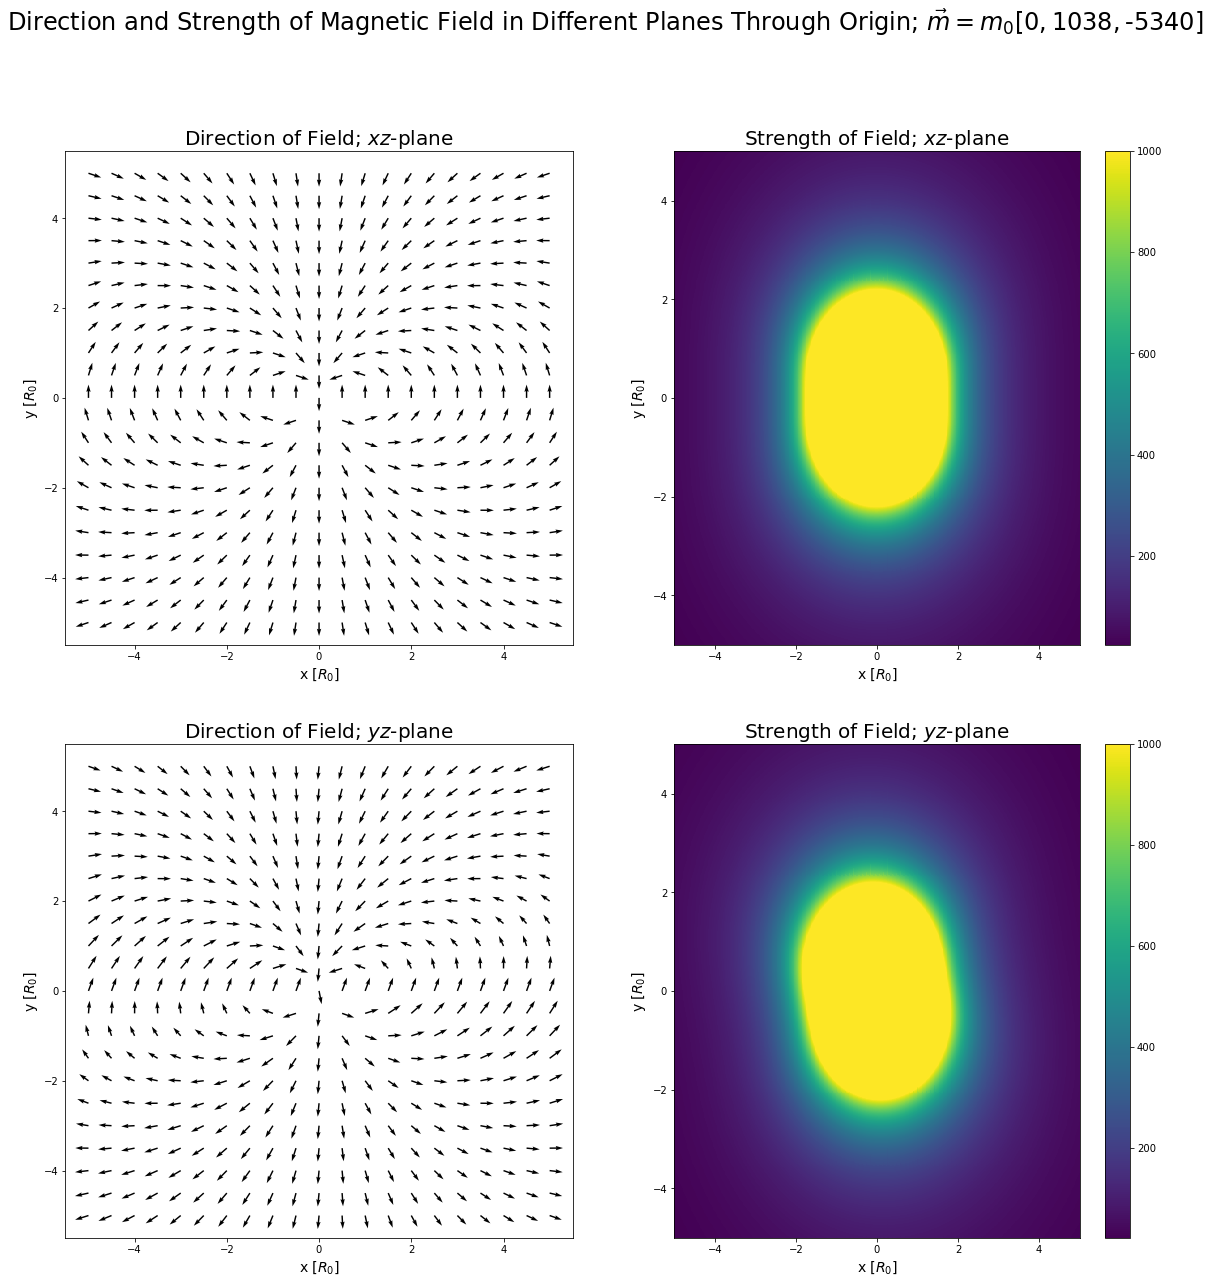
\includegraphics[scale=.28]{Images/dipolePlanes.png}
    \caption{Direction and strength of the magnetic field of our dipole in the $xz$-plane (upper images) and in the $yz$-plane (lower images).}
    \label{fig:dipolePlanes}
\end{figure}

\noindent Most apparent is the fact that the magnetic field is tilted in the $yz$-plane, which corresponds to the tilt we imposed on our dipole moment. This tilt can also be seen in Figure \ref{fig:dipoleField}, though it is harder to see. The tilt is present in the plot of the $xz$-plane too since the arrows in the top half of the plot for the $xz$-plane point steeper towards the center than the arrows in the bottom half point away from the center. Another note about Figure \ref{fig:dipolePlanes} is that the strength of the field, though exaggerated in the plots, has an elliptical shape along the dipole moment. This corresponds to the real behaviour of a dipole